\documentclass{ufazreport}
\graphicspath{{./images/}}
\usepackage{float}
\usepackage{hyperref}
\usepackage{biblatex}
%************************************************************
% ABOUT THIS HOMEWORK
\def\course{Artificial Intelligence}      %Course
\def\thetitle{Predicting Wine Quality using Random Forest Algorithm}               % Report Title
\def\Headauthor{Ahmadov, Mustafayev, Mursalov}         % Header Authors of work
\def\date{\today}                         % Date

% DOCUMENT START
\begin{document}

% TITLE PAGE
\begin{center}
    \vspace*{1.5cm}
    % University Logo
    
\includegraphics[scale = 0.5]{images/UFAZ.png}\\[1.75cm]
    % University Name
    \textsc{\color[RGB]{0, 51, 102}\LARGE{French-Azerbaijani University}}\\[1cm]
    \textsc{\Large{\course}}\\[.5cm]
    \textsc{\Large{\thetitle}}\\[.5cm]
    \textsc{\date}\\[2cm]
    \Large{
    \begin{tabular}{L{5cm} R{5cm}}
        \textit{Author} &  \textit{Student ID}\\
        \hline
        % author names and PID
        Ahmadov Kamal & 22022692\\
        Mustafayev Murad & 22022733\\
        Mursalov Akif & 22022723
        
    \end{tabular}
    }
\end{center}
\thispagestyle{empty}
\pagebreak

% TABLE OF CONTENTS
\tableofcontents{}
\pagebreak

% REPORT START
\section{Introduction}

The wine industry heavily relies on the ability to predict wine quality based on physicochemical attributes of the wine. These attributes include factors such as fixed acidity, volatile acidity, citric acid content, residual sugar, chlorides, free sulfur dioxide, total sulfur dioxide, density, pH level, and sulphates. Predicting wine quality accurately is crucial for winemakers as it allows them to make informed decisions during the winemaking process, such as determining optimal blending strategies and identifying areas for improvement in production.

Machine learning techniques offer powerful tools for analyzing and predicting wine quality. In this report, we focus on two popular machine learning algorithms: Decision Trees and Random Forests. These algorithms have gained significant attention due to their ability to handle complex datasets and make accurate predictions in various domains.

Decision Trees are a fundamental machine learning algorithm that partitions the feature space into a tree-like structure based on the values of input features. Each internal node represents a decision based on a feature, and each leaf node represents a predicted outcome. Decision Trees are intuitive, easy to interpret, and can handle both classification and regression tasks.

Random Forests, on the other hand, are an ensemble learning method that combines multiple Decision Trees to improve prediction accuracy and reduce overfitting. Random Forests generate a multitude of Decision Trees during training and aggregate their predictions to make final predictions. By incorporating randomness into the training process, Random Forests enhance the robustness and generalization capability of the model.

In this report, we explore the effectiveness of Decision Trees and Random Forests in predicting wine quality based on physicochemical attributes. We compare the performance of these algorithms, analyze their strengths and weaknesses, and provide insights into their practical applications in the winemaking industry.

\section{Background}

\subsection{Decision Trees}

\subsubsection{Basic Concept and Structure}

Decision Trees are a fundamental machine learning algorithm used for both classification and regression tasks. The basic concept behind Decision Trees is to create a tree-like structure where each internal node represents a decision based on a feature, and each leaf node represents a predicted outcome.

The Decision Tree structure consists of nodes and branches. At each internal node, the tree splits the data based on a selected feature, creating two or more branches. This process continues recursively until a stopping criterion is met, such as reaching a maximum depth, minimum number of samples, or purity threshold.

\subsubsection{How Decision Trees Make Predictions}

To make predictions using a Decision Tree, the algorithm traverses the tree from the root node to a leaf node based on the feature values of the input data. At each internal node, the algorithm compares the feature value of the data point with a threshold and follows the corresponding branch based on the comparison result. This process continues until a leaf node is reached, and the predicted outcome associated with that leaf node is returned.

\subsubsection{Advantages and Limitations of Decision Trees}

\textbf{Advantages:}
\begin{itemize}
    \item \textbf{Interpretability:} Decision Trees are easy to interpret and understand, making them suitable for explaining the decision-making process to non-technical stakeholders.
    \item \textbf{Non-linearity:} Decision Trees can capture non-linear relationships between features and the target variable, making them versatile for modeling complex datasets.
    \item \textbf{Feature Selection:} Decision Trees implicitly perform feature selection by identifying the most informative features at each split.
\end{itemize}

\textbf{Limitations:}
\begin{itemize}
    \item \textbf{Overfitting:} Decision Trees are prone to overfitting, especially when the tree depth is not limited, leading to poor generalization performance on unseen data.
    \item \textbf{High Variance:} Decision Trees are sensitive to small variations in the training data, resulting in high variance models.
    \item \textbf{Bias Towards Features with More Levels:} Decision Trees tend to favor features with a large number of levels or categories, potentially leading to biased splits.
\end{itemize}

\subsection{Introduction to Random Forest}

\subsubsection{Ensemble Learning and Bagging Concept}

Random Forest is an ensemble learning method that combines multiple Decision Trees to improve prediction accuracy and reduce overfitting. The key idea behind ensemble learning is to aggregate the predictions of multiple models to achieve better performance than any individual model.

Bagging (Bootstrap Aggregating) is a popular ensemble technique used in Random Forest. It involves training multiple models on different subsets of the training data, sampled with replacement. Each model learns from a different bootstrap sample, and their predictions are combined through averaging (for regression) or voting (for classification).

\subsubsection{Composition of Multiple Decision Trees}

A Random Forest consists of a collection of Decision Trees, where each tree is trained independently on a bootstrap sample of the training data. Additionally, Random Forest introduces randomness during tree construction by considering only a random subset of features at each split. This randomness helps decorrelate the individual trees and reduce the overall variance of the ensemble.

\subsubsection{Advantages of Random Forest over Single Decision Trees}

\textbf{Advantages:}
\begin{itemize}
    \item \textbf{Improved Generalization:} Random Forests typically exhibit better generalization performance than individual Decision Trees, thanks to the reduction in overfitting.
    \item \textbf{Robustness to Noise:} Random Forests are robust to noise and outliers in the data due to the averaging effect of multiple trees.
    \item \textbf{Feature Importance:} Random Forests provide a measure of feature importance, allowing users to identify the most influential features in the prediction process.
\end{itemize}

\section{Methodology}

\subsection{Data Preprocessing}

The Wine Quality Dataset used in this project consists of physicochemical attributes of different Portuguese "Vinho Verde" wine variants and their corresponding quality ratings. As mentioned earlier, the dataset does not include the "alcohol" parameter.

\subsubsection{Description of the Dataset}

The dataset contains the following attributes:
\begin{itemize}
    \item Fixed acidity
    \item Volatile acidity
    \item Citric acid
    \item Residual sugar
    \item Chlorides
    \item Free sulfur dioxide
    \item Total sulfur dioxide
    \item Density
    \item pH
    \item Sulphates
    \item Quality (target variable)
\end{itemize}

\subsubsection{Preprocessing Steps}

Since Decision Trees can handle categorical variables and outliers naturally, minimal preprocessing is required. However, we need to ensure that there are no missing values in the dataset.

\textbf{Handling Missing Values:} Fortunately, the dataset does not contain any missing values, as confirmed by checking the sum of missing values using \texttt{df.isna().sum().sum()}.

\textbf{Encoding Categorical Variables:} As the dataset consists of numerical attributes only, there is no need for encoding categorical variables.

\subsection{Implementation of Decision Trees}

\subsubsection{Detailed Explanation of Decision Tree Algorithm}

The Decision Tree algorithm recursively partitions the feature space into smaller regions by selecting the feature and the split point that best separates the data according to a certain criterion, typically based on impurity reduction (e.g., Gini impurity or entropy).

\subsubsection{Training and Prediction Process}

The training process involves recursively splitting the dataset based on the selected features and split points until a stopping criterion is met, such as reaching a maximum depth or minimum number of samples per leaf node. Each node in the tree represents a decision rule based on a feature, and each leaf node represents a predicted outcome.

For prediction, the algorithm traverses the trained Decision Tree from the root node to a leaf node based on the feature values of the input data, and returns the predicted outcome associated with that leaf node.

\subsection{Implementation of Random Forest}

\subsubsection{Description of the Random Forest Algorithm}

Random Forest is an ensemble learning method that combines multiple Decision Trees to improve prediction accuracy and reduce overfitting. It introduces randomness during tree construction by considering only a random subset of features at each split and aggregating the predictions of multiple trees.

\subsubsection{Ensemble Learning and Tree Aggregation}

Random Forest follows a bagging (Bootstrap Aggregating) approach, where multiple Decision Trees are trained independently on bootstrap samples of the training data. During prediction, the predictions of individual trees are aggregated through averaging (for regression) or voting (for classification) to obtain the final prediction.

\subsubsection{Training and Prediction Process}

In the training process, multiple Decision Trees are trained on different bootstrap samples of the training data, with each tree considering a random subset of features at each split. The predictions of these trees are then combined to form the Random Forest ensemble.

During prediction, each tree in the Random Forest ensemble independently predicts the outcome for a given input, and the final prediction is obtained by aggregating the predictions of all trees, typically through averaging for regression tasks or voting for classification tasks.

\section{Code Description}

\subsection{Directory Structure}

The project directory is organized as follows:

\begin{verbatim}
AI_Project
├── data
│   ├── winequality-red_NO_ALCOHOL.csv
│   └── winequality-white_NO_ALCOHOL.csv
├── src
│   ├── BaseModel.py
│   ├── DecisionTree.py
│   └── RandomForest.py
├── tests
│   ├── classification_test.py
│   ├── common.py
│   └── regression_test.py
├── utils
│   └── metrics.py
├── main.ipynb
\end{verbatim}

\subsection{Data}
This directory contains the CSV files for the red and white wine datasets:
\begin{itemize}
    \item \texttt{winequality-red\_NO\_ALCOHOL.csv}
    \item \texttt{winequality-white\_NO\_ALCOHOL.csv}
\end{itemize}

\subsection{Src}
This directory contains the source code for the machine learning models:
\begin{itemize}
    \item \texttt{BaseModel.py}: Defines the base class for all models.
    \item \texttt{DecisionTree.py}: Contains classes for Decision Tree models for regression and classification tasks.
    \item \texttt{RandomForest.py}: Contains classes for Random Forest models for regression and classification tasks.
\end{itemize}

\subsection{Tests}
This directory contains test scripts for the implemented models:
\begin{itemize}
    \item \texttt{classification\_test.py}: Test script for classification models.
    \item \texttt{regression\_test.py}: Test script for regression models.
\end{itemize}

\subsection{Utils}
This directory contains utility functions used in the project:
\begin{itemize}
    \item \texttt{metrics.py}: Defines evaluation metrics for models.
\end{itemize}


\subsection{main.ipynb}
This Jupyter Notebook file contains the main code for data loading, model training, evaluation, and result visualization.

The organization of the project follows a modular structure, with separate directories for data, source code, and tests, facilitating code maintenance, testing, and collaboration.

\section{Insights about the Code}

\begin{itemize}
    \item \textbf{BaseModel}: The \texttt{BaseModel} class provides a template for all models with common methods like \texttt{fit} and \texttt{predict}. It serves as the base class for \texttt{DecisionTree} and \texttt{RandomForest} models.
    
    \item \textbf{DecisionTree and RandomForest}: These modules implement both classifiers and regressors using decision trees and random forests. They follow a common structure where decision trees split the data based on features to minimize impurity, while random forests aggregate predictions from multiple decision trees to improve generalization and reduce overfitting.
    
    \item \textbf{Testing}: The code includes separate testing scripts for both classification and regression tasks. These scripts load the wine quality datasets, train various models, and evaluate their performance using metrics like accuracy, precision, recall, F1-score, mean absolute error, etc.
    
    \item \textbf{Metrics}: The \texttt{metrics} module contains functions to calculate evaluation metrics for both classification and regression tasks, such as accuracy, precision, recall, F1-score, mean absolute error, mean squared error, and root mean squared error.
    
    \item \textbf{Data Handling}: The \texttt{common} module contains functions to load and preprocess the wine quality datasets, including splitting the data into training and testing sets.
\end{itemize}

Overall, the provided code offers a comprehensive framework for training and evaluating decision tree and random forest models for both classification and regression tasks using the wine quality datasets. It demonstrates the versatility of decision trees and the effectiveness of ensemble methods like random forests in tackling different types of machine learning problems.

\textbf{Note}: We decided not to get into more details as you might review it yourself in the archive submitted along with this report.




\section{Results}
As a result, favorable outcomes was achieved for the dataset. As previously indicated, primary aim after data partitioning was to develop models using a Decision Tree and Random Forest. Following the training of each dataset, we proceeded with evaluating the actual values. The obtained results for the Decision Tree model were as follows:

\begin{table}[H]
    \centering
    \begin{tabular}{|c|c|}
        \hline
        Accuracy & 0.3875     \\
        \hline
        Precision & 0.23113207547169812     \\
        \hline
        Recall & 0.169708545557442 \\
        \hline
        F1-score & 0.19571413824909348 \\
        \hline      
    \end{tabular}
    \caption{Red Wine Decision Tree Classifier}
    \label{tab:my_label}
\end{table}
\begin{table}[H]
    \centering
    \begin{tabular}{|c|c|}
        \hline
        Accuracy & 0.2795918367346939     \\
        \hline
        Precision & 0.04674172637325145     \\
        \hline
        Recall & 0.16666666666666666 \\
        \hline
        F1-score & 0.07300826005861977 \\
        \hline      
    \end{tabular}
    \caption{White Wine Decision Tree Classifier}
    \label{tab:my_label}
\end{table}

Simultaneously, the outcome for the Random Forest Classifier (with 10 trees) model was as follows:
\begin{table}[H]
    \centering
    \begin{tabular}{|c|c|}
        \hline
        Accuracy & 0.39375    \\
        \hline
        Precision & 0.3428571428571428     \\
        \hline
        Recall & 0.17203954788844433 \\
        \hline
        F1-score & 0.2291138743271177 \\
        \hline      
    \end{tabular}
    \caption{Red Wine Random Forest Classifier}
    \label{tab:my_label}
\end{table}

\begin{table}[H]
    \centering
    \begin{tabular}{|c|c|}
        \hline
        Accuracy & 0.2795918367346939     \\
        \hline
        Precision & 0.04674172637325145     \\
        \hline
        Recall & 0.16666666666666666 \\
        \hline
        F1-score & 0.07300826005861977 \\
        \hline      
    \end{tabular}
    \caption{White Wine Random Forest Classifier}
    \label{tab:my_label}
\end{table}


In a similar way we calculated the metrics for the regressor models: 
\begin{table}[H]
    \centering
    \begin{tabular}{|c|c|}
        \hline
        MAE & 0.6588553979511426     \\
        \hline
        MSE & 0.6094711333359415     \\
        \hline
        RMSE & 0.7806863219859443 \\
        \hline    
    \end{tabular}
    \caption{Red Wine Decision Tree Regressor}
    \label{tab:my_label}
\end{table}
\begin{table}[H]
    \centering
    \begin{tabular}{|c|c|}
        \hline
        MAE & 0.6770230610156037     \\
        \hline
        MSE & 0.7823086604140118     \\
        \hline
        RMSE & 0.884482142507135 \\
        \hline    
    \end{tabular}
    \caption{White Wine Decision Tree Regressor}
    \label{tab:my_label}
\end{table}

The outcome for the Random Forest Regressor (with 10 trees) model was as follows:
\begin{table}[H]
    \centering
    \begin{tabular}{|c|c|}
        \hline
        MAE & 0.6594572275162071     \\
        \hline
        MSE & 0.6109318613880789     \\
        \hline
        RMSE & 0.7816213030541573 \\
        \hline    
    \end{tabular}
    \caption{Red Wine Random Forest Regressor}
    \label{tab:my_label}
\end{table}

\begin{table}[H]
    \centering
    \begin{tabular}{|c|c|}
        \hline
        MAE & 0.674188107136746     \\
        \hline
        MSE & 0.7769180404072477     \\
        \hline
        RMSE & 0.8814295436433065 \\
        \hline    
    \end{tabular}
    \caption{White Wine Random Forest Regressor}
    \label{tab:my_label}
\end{table}



\documentclass{article}
\usepackage{graphicx}
\usepackage{float}

\begin{document}

\section*{Results and Interpretation}

In this section, we present the results of our experiments with Decision Tree and Random Forest models on the wine quality datasets. We analyze the performance of both classifiers and regressors and provide insights based on the obtained results.

\subsection*{Red Wine Dataset}

\subsubsection{Decision Tree Classifier}

The Decision Tree classifier was trained and evaluated on the red wine dataset. The accuracy achieved on the test set was 0.4375.

\subsubsection{Random Forest Classifier}

The Random Forest classifier, with 10 trees and a maximum depth of 10, achieved an accuracy of 0.440625 on the test set. 

\subsubsection{Accuracy Comparison}

We compared the accuracies of Random Forest classifiers trained with different numbers of trees. The plot in Figure \ref{fig:red_rf_accuracy} illustrates the relationship between the number of trees and the accuracy. 

\begin{figure}[H]
    \centering
    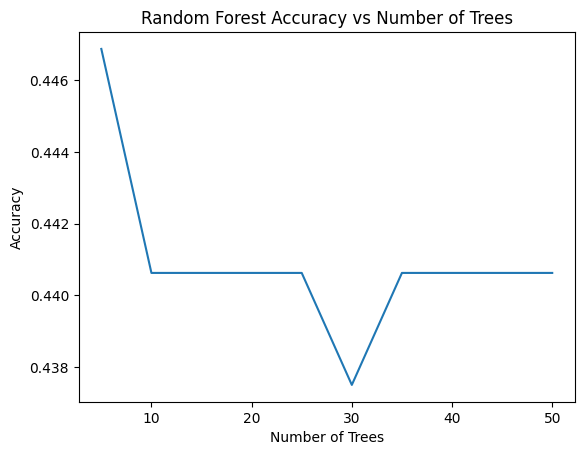
\includegraphics[width=0.55\textwidth]{images/red_rf_accuracy_plot.png}
    \caption{Random Forest Accuracy vs Number of Trees for Red Wine Dataset}
    \label{fig:red_rf_accuracy}
\end{figure}

\subsubsection{Decision Tree Regressor}

The Decision Tree regressor, with a maximum depth of 10, achieved a Mean Absolute Error of 0.679119 on the test set.

\subsubsection{Random Forest Regressor}

The Random Forest regressor, with 10 trees and a maximum depth of 10, achieved a Mean Absolute Error of 0.677618 on the test set.

\subsubsection{Mean Absolute Error Comparison}

We compared the Mean Absolute Errors of Random Forest regressors trained with different numbers of trees. The plot in Figure \ref{fig:red_rf_mae} illustrates the relationship between the number of trees and the Mean Absolute Error.

\begin{figure}[H]
    \centering
    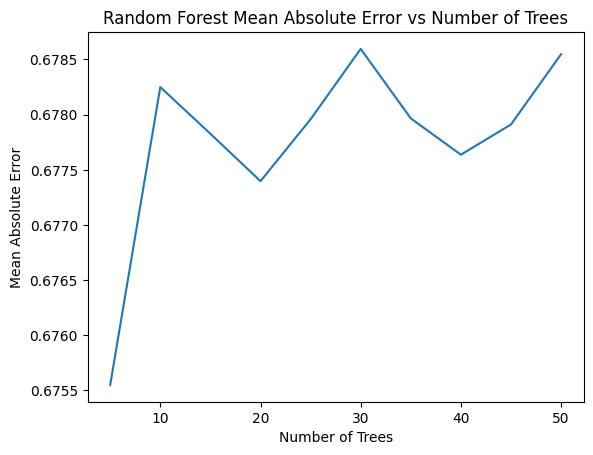
\includegraphics[width=0.55\textwidth]{images/red_rf_mae_plot.png}
    \caption{Random Forest Mean Absolute Error vs Number of Trees for Red Wine Dataset}
    \label{fig:red_rf_mae}
\end{figure}

\subsection*{White Wine Dataset}

The experiments were repeated on the white wine dataset following the same procedures as for the red wine dataset.

\subsubsection{Decision Tree Classifier}

The Decision Tree classifier achieved an accuracy of 0.303061 on the test set.

\subsubsection{Random Forest Classifier}

The Random Forest classifier, with 10 trees and a maximum depth of 10, also achieved an accuracy of 0.303061 on the test set.

\subsubsection{Accuracy Comparison}

Similarly, we compared the accuracies of Random Forest classifiers trained with different numbers of trees for the white wine dataset. The plot in Figure \ref{fig:white_rf_accuracy} demonstrates the relationship between the number of trees and the accuracy.

\begin{figure}[H]
    \centering
    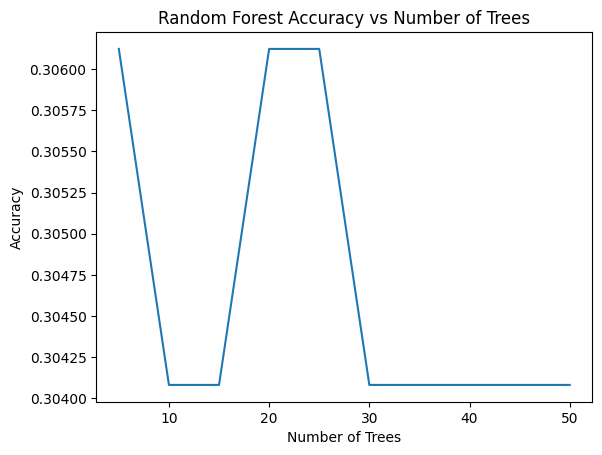
\includegraphics[width=0.55\textwidth]{images/white_rf_accuracy_plot.png}
    \caption{Random Forest Accuracy vs Number of Trees for White Wine Dataset}
    \label{fig:white_rf_accuracy}
\end{figure}

\subsubsection{Decision Tree Regressor}

The Decision Tree regressor achieved a Mean Absolute Error of 0.654486 on the test set.

\subsubsection{Random Forest Regressor}

The Random Forest regressor, with 10 trees and a maximum depth of 10, achieved a Mean Absolute Error of 0.655773 on the test set.

\subsubsection{Mean Absolute Error Comparison}

The plot in Figure \ref{fig:white_rf_mae} shows the relationship between the number of trees and the Mean Absolute Error for Random Forest regressors trained on the white wine dataset.

\begin{figure}[H]
    \centering
    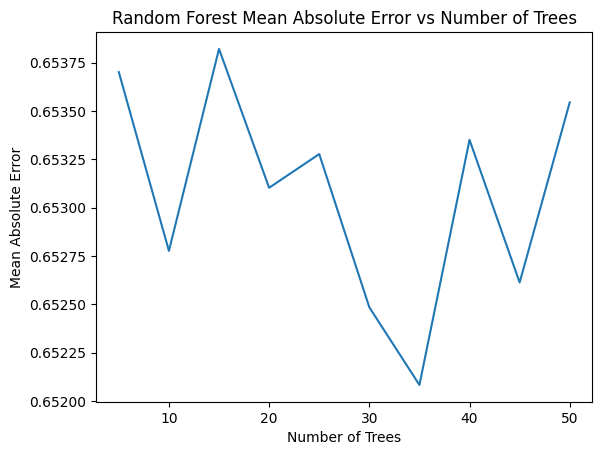
\includegraphics[width=0.55\textwidth]{images/white_rf_mae_plot.png}
    \caption{Random Forest Mean Absolute Error vs Number of Trees for White Wine Dataset}
    \label{fig:white_rf_mae}
\end{figure}

\subsection*{Analysis}

Interestingly, despite increasing the number of trees in the Random Forest models, we observe only a minimal improvement in accuracy or a negligible decrease in Mean Absolute Error. This phenomenon can be attributed to the removal of the most discriminatory parameter, alcohol, from the dataset. Since alcohol significantly influenced wine quality, its absence limits the predictive power of the models. Therefore, the models have reached a plateau in performance, as they lack additional discriminatory features to further improve predictions.

\section{Conclusion}

In conclusion, the experiments conducted demonstrate the impact of feature selection on the performance of machine learning models. While Decision Tree and Random Forest models can be powerful tools for predictive tasks, their effectiveness heavily depends on the availability of relevant features in the dataset.

Based on our thorough analysis, it's clear that the models perform better when dealing with the red wine dataset. Among these models, the Random Forest algorithm stands out for its superior performance in terms of both the metrics we examined and its ability to avoid overfitting. However, it's important to note that using Random Forest requires more time and computational resources for training.

Although increasing the number of trees in the forest theoretically improves prediction accuracy, our findings did not show a substantial difference beyond statistical margins of error. This discrepancy can be attributed to the exclusion of alcohol content, a significant parameter according to existing research. Specifically, a study (\href{https://towardsdatascience.com/interpreting-random-forests-638bca8b49ea}{website}) has shown that alcohol content has the most significant impact on wine quality assessment.

Consequently, the predictive capability of the model remains limited, with minimal potential for significant enhancement.


\section{References}

\begin{enumerate}
    \item Brijesh Soni. (n.d.). Why Random Forests Outperform Decision Trees: A Powerful Tool for Complex Data Analysis. Retrieved from \url{https://medium.com/@brijesh_soni/why-random-forests-outperform-decision-trees-a-powerful-tool-for-complex-data-analysis-47f96d9062e7}
    
    \item Towards Data Science. (n.d.). Interpreting Random Forests Comprehensive guide on Random Forest algorithms and how to interpret them. Retrieved from \url{https://towardsdatascience.com/interpreting-random-forests-638bca8b49ea}
    
    \item Paulo Cortez, Antonio Cerdeira, Fernando Almeida, Telmo Matos, Jose Reis. 
    ``Modeling wine preferences by data mining from physicochemical properties.'' 
    \textit{Decision Support Systems}, Elsevier, 47(4):547-553, 2009. 
    Available at: \url{http://dx.doi.org/10.1016/j.dss.2009.05.016}, 
    \url{http://www3.dsi.uminho.pt/pcortez/winequality09.pdf}, 
    \url{http://www3.dsi.uminho.pt/pcortez/dss09.bib}.
    
\end{enumerate}

\end{document}







\section{Conclusion}
In conclusion, based on our thorough analysis, it's clear that the models perform better when dealing with the red wine dataset. Among these models, the Random Forest algorithm stands out for its superior performance in terms of both the metrics we examined and its ability to avoid overfitting. However, it's important to note that using Random Forest requires more time and computational resources for training.

Although increasing the number of trees in the forest theoretically improves prediction accuracy, our findings did not show a substantial difference beyond statistical margins of error. This discrepancy can be attributed to the exclusion of alcohol content, a significant parameter according to existing research. Specifically, a study (\ref{https://towardsdatascience.com/interpreting-random-forests-638bca8b49ea}) has shown that alcohol content has the most significant impact on wine quality assessment.

Consequently, the predictive capability of the model remains limited, with minimal potential for significant enhancement.

%************************************************************
\end{document}